\appendices
\section{Generation Prompts and Recorded Settings}
\label{app:prompts}
The supplementary artifact provides literal Chinese templates exported from the prompt builders, their SHA-256 hashes, and English translations. The translations below describe the same tasks and response fields; they are not presented as the language used in the historical calls. The archive contains the parsed responses and deletion fragments, but not each fully rendered request or a complete historical decoding configuration.

\subsection{Deletion Completion Prompt}
\label{app:prompt_deletion}
The actual builder asks: ``You are an expert in rule extraction for government-service knowledge graphs. Some phrases have been randomly removed from a service document. Read the original and the incomplete version, infer the missing rule information using the context and domain knowledge, and express it as constraints for graph validation. Return only JSON following the supplied schema.'' The request includes the service item, original source, incomplete source, and deleted fragments. It asks for general types and relations rather than only instance names.

The JSON fields are \texttt{strategy}, \texttt{service\_item}, \texttt{analysis}, \texttt{removed\_fragments}, \texttt{missing\_rule\_candidates}, and \texttt{proposed\_rules}. The latter contains the seven candidate categories described below. This call is made once per document; ten repeated entity masks and frequency-threshold filtering are not part of the archived runner.

\subsection{Augmentation Expansion Prompt}
\label{app:prompt_augmentation}
The actual builder asks: ``You are an expert in rule extraction for government-service knowledge graphs. Propose no more than three reasonable supplementary clauses for the document, while preserving plausibility and compliance, and infer graph-validation rules from the additions. Return only JSON following the supplied schema.'' The request includes the service item and original text, and asks for reusable rather than instance-specific candidates.

Its response contains \texttt{strategy}, \texttt{service\_item}, \texttt{analysis}, \texttt{added\_clauses}, and \texttt{proposed\_rules}. The schema categories are entity types, relationship types, forbidden type-relation patterns, allowed type-relation patterns, hierarchy statements, geographical hierarchy patterns, and procedural statements. Both calls use the same candidate categories.

\subsection{Defaults and Missing Metadata}
The script defaults are Qwen3-32B, temperature 0.2, up to five deleted spans of at most six characters, and at most three supplementary clauses. The client does not explicitly set a completion-token cap or top-$p$. Historical per-call records contain the document identifier, service item, strategy, parsed result, and deletion fragments when applicable. They do not certify that every invocation used the current defaults. The separate 45-document extraction experiment records Qwen3.8-27B-no-thinking.

\section{RuleTest-94 and Direct Execution}
\label{app:testset}
The suite contains 30 clean and 64 defective records: 10 hierarchy reversals, 10 absurd relations, 10 reverse-supervision cases, 30 procedural or missing-field cases, and four specialist cases. The revised scorer reads \texttt{expected\_detection} directly: \texttt{pass} is negative, while \texttt{fail} and \texttt{specialist\_miss} are positive. It does not derive labels by running the detector under evaluation. These are designed labels without independent annotator identities or disagreement records.

The hand-implemented family union still detects all 64 defects without flagging the 30 clean records under these stored labels. Its precision Wilson interval is $[0.943,1.000]$ and specificity interval $[0.886,1.000]$. This family-union score is distinct from the direct execution of archived candidates reported in Section~\ref{sec:rule_execution_audit}.

\label{app:rule_format}
Each directly compiled constraint has an identifier, allowed/forbidden kind, exact subject-type/relation/object-type pattern, and a list of original source locations. Pattern membership determines whether a record matches; allowed patterns do not define a closed-world whitelist. Contradictory permission and prohibition yield an explicit abstention. Unsupported natural-language candidates are retained without invented formal interpretations.

\section{Typed-Document Generation Pilot}
\label{app:docred_pilot}
We prepare a separate source-grouped DocRED~\cite{ref_docred} sample with
180 training, 60 development and 60 test documents from the original annotated
training corpus. Entity identities and mention types are given. Public source
inputs and relation references are stored separately; generation and policy
observations do not read reference relations.

A fixed ten-document development pilot collects two rule responses and one
natural extraction per document using Gemma. Its 30 outputs require 34 actual
requests including retries. All twenty rule responses parse, yielding 263
compiled candidates: 156 allowed and 107 forbidden patterns. One extraction
response fails the frozen parser and remains an empty graph; the others yield
106 executable relations. Five two-document episodes are replayed under
immediate stop and four fixed acquisition/repair schedules. No schedule deletes
a record, and all schedules produce the same final graph within each episode.
The pilot therefore identifies a coverage gap between the generated forbidden
patterns and these natural extraction outputs. Type compatibility alone does
not establish factual correctness. Formal learned scheduling on this new
corpus has not started; the development records and implementation are archived
in \texttt{exps/paper2\_docred}.

\subsection{Source-Evidence Development Test}
\label{app:docred_v2}
A separate version retains dual-strategy generation and the four-action scheduler, and adds document-scoped source constraints. Each candidate marks a concrete record as supported, contradicted, or insufficient. The compiler validates an exact quote in a numbered original sentence and records its character offsets. Hypothetical augmentation clauses cannot supply evidence. Insufficient evidence causes abstention. Conflicting support and contradiction also cause abstention; type compatibility alone cannot cancel a source contradiction.
For this version, let $V(g;R)$ be the set of nonconflicting violations and $N$ the initial record count (with denominator one for an empty input). We use $G(g;R)=1-|V(g;R)|/N$ and coverage $C$ over the initial records. The graph-change term compares both graphs under the updated rules:
\begin{align}
r_t={}&0.5\left[G(g_{t+1};R_{t+1})-G(g_t;R_{t+1})\right] \nonumber\\
&+0.5(C_{t+1}-C_t)-0.004a_t \nonumber\\
&-0.00002d_t-|V_{\mathrm{edit},t}|/N,
\end{align}
where $a_t$ counts acquired responses, $d_t$ counts removed records, and $V_{\mathrm{edit},t}=V(g_{t+1};R_{t+1})\setminus V(g_t;R_{t+1})$. Thus acquisition can reveal a violation without being charged for creating it. A two-record synthetic counterexample changes the discounted acquire--repair return from $-0.266519$ to $0.483481$ at discount $0.95$. This is an accounting check, not an empirical quality gain. Source support is still a model judgment; quote validation does not prove its meaning.
Before calls, we fix the first ten development pairs (20 documents). Each pair contains one reference graph and one reference graph with added endpoint or relation substitutions, numbering $\lceil0.2|G^*|\rceil$. References are used in construction and scoring, not in prompts, observations, or reward. The observations contain 14 public summaries and an action mask; they are not asserted to be a sufficient Markov state. Each episode allows four response acquisitions, two per strategy, and ten steps. The removal operator retains the emptying guard.
\begin{table}[t]
\centering
\caption{Source-evidence development diagnostics on ten fixed document pairs. F1 and preservation are episode means. Lost counts removed reference facts. No learned policy is evaluated.}
\label{tab:docred_source_pilot}
\small
\begin{tabular}{lrrr}
\hline
Schedule & F1 (\%) & Preserved (\%) & Lost \\
\hline
Stop & 94.42 & 100.00 & 0 \\
Acquire then repair & 94.59 & 98.34 & 4 \\
Repair when feasible & 91.63 & 93.51 & 18 \\
Uniform feasible & 94.42 & 100.00 & 0 \\
\hline
\end{tabular}
\end{table}
The 40 outputs require 40 actual Gemma requests. They compile to 357 type rules, 61 source-support rules, and 6 source-contradiction rules. Source constraints trigger removals in 4 of ten episodes. The pre-call expansion gate requires this in at least two episodes and at least one fixed schedule to improve mean reference F1 while preserving at least 99\% of reference facts.
The development gate is not met, so this version is not expanded to learned-policy training or held-out evaluation.
These results measure reference recovery and removal of injected items. Independent assessment of natural relations and edits remains pending. Cached schedule replay makes zero API calls; generation requests are counted separately.
\begin{figure*}[t]
\centering
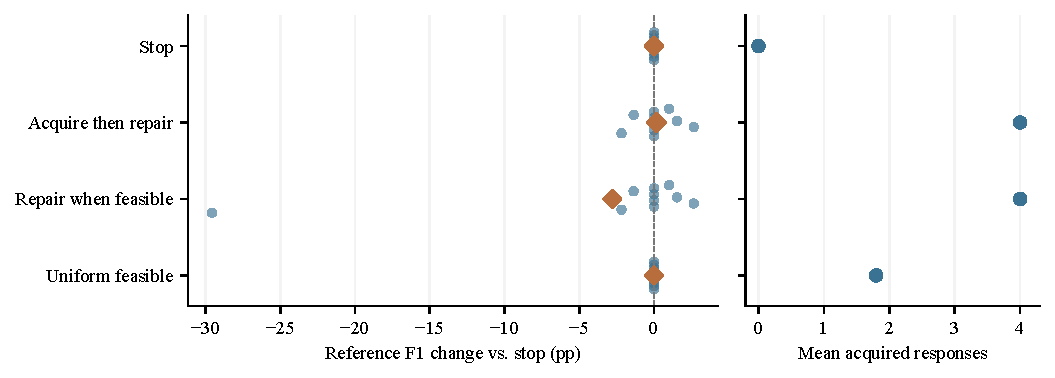
\includegraphics[width=0.94\textwidth]{figure/experiments/docred_source_pilot.pdf}
\caption{Source-evidence development replay. Small points show ten episode-level F1 changes from stop; diamonds show their mean. The right panel shows cached response acquisitions.}
\label{fig:docred_source_pilot}
\end{figure*}

\paragraph{Second development round.}
We retain the same twenty documents, compiler, reward, budget, and gate.
The only changes add readable entity names and clarify property direction,
historical roles, and the distinction between absent and contradictory evidence.
Forty further requests complete without transport failures; 38 responses pass
the fixed rule parser. They yield 243 type rules and 14 source-support rules,
but no executable source-contradiction rule. Both acquire-then-repair and
repair-when-feasible reach 95.69\% reference F1, compared with 94.42\% for stop.
Each removes seven of 31 injected items and loses no reference fact.
All seven removals come from type constraints. Source constraints therefore
fail the required repair-effect gate, and the two development rounds end
without expanded training or a held-out generated-rule policy evaluation.
The compiler also rejects 120 and 257 type candidates in the two rounds
that copy the example string \texttt{allowed or forbidden} instead of selecting
one kind. The fixed parser is not relaxed after collection.
The first round's harmful deletions and the second round's empty source-repair
coverage are both retained. These checks show why executable quotation and
correct scheduling interfaces alone do not establish useful source constraints.

\begin{figure*}[t]
\centering
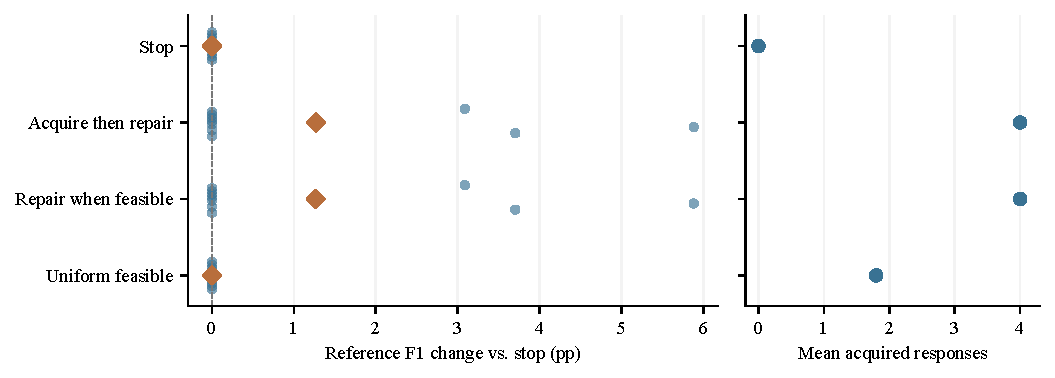
\includegraphics[width=0.94\textwidth]{figure/experiments/docred_source_pilot_round2.pdf}
\caption{Second and final development round on the same ten pairs.
F1 improves under the two repair schedules without reference losses, but all
removals use type constraints. Repeated rounds are not new test documents.}
\label{fig:docred_source_round2}
\end{figure*}


\section{Independent Rule-Feasibility Follow-up}
\label{app:new_rule_feasibility}
After closing the two-round study, we freeze a separate development protocol
with twenty other documents. We take the first ten pairs in the original
development order whose members occur in neither prior pilot membership nor
prior response logs. Selection uses no content or outcome scores. Each pair
contains one reference graph and one graph with injected records, totaling
226 reference facts and 28 injected items. These inputs measure controlled
reference recovery; an unannotated relation is not automatically a false fact.

The prompts supply concrete JSON enum examples and a schema limiting output
to twenty rules and three supplementary clauses. Duplicate keys, invalid
enums and oversized lists invalidate the whole response. Valid candidates
still pass the original vocabulary and quotation checks. Forty requests to
\texttt{google/gemma-4-26B-A4B-it}, with temperature zero and a 4,000-token
completion cap, complete without transport failures or retries. One response
exceeds the rule limit and remains an empty packet. The 39 schema-valid
responses yield 109 allowed and 36 forbidden type rules, 256 source-support
rules, and six source-contradiction rules. All six contradictions come from
deletion. The compiler also records 163 insufficient-evidence abstentions
and rejects nineteen candidates whose quotes do not match the original text.

\begin{table}[t]
\centering
\caption{Independent development follow-up on ten document pairs.
F1, reference preservation (Pres.) and acquired packets are pair means;
removed injected items (Rem.) and lost reference facts (Lost) are totals.
Both-bank schedules share the same final graphs.}
\label{tab:new_rule_feasibility}
\small
\setlength{\tabcolsep}{3pt}
\begin{tabular}{lrrrrr}
\toprule
Schedule & F1 (\%) & Pres. (\%) & Rem. & Lost & Packets \\
\midrule
Stop & 94.02 & 100.00 & 0 & 0 & 0.0 \\
Both banks & 96.63 & 98.14 & 17 & 4 & 4.0 \\
Deletion only & 96.63 & 98.14 & 17 & 4 & 2.0 \\
Augmentation only & 94.24 & 100.00 & 1 & 0 & 2.0 \\
Uniform feasible & 95.58 & 100.00 & 8 & 0 & 2.1 \\
\bottomrule
\end{tabular}
\end{table}

The eight predefined schedules are stop, both acquisition orders with
immediate or deferred repair, the two single-bank schedules, and uniform
sampling of feasible actions including stop. Their eighty replays agree
with exhaustive enumeration of 384 terminal paths. Random scheduling uses
one frozen seed per pair. The acquire-then-repair F1 difference from stop is
2.61 percentage points, with a descriptive paired-bootstrap 95\% interval
of $[0.81,4.30]$ from 10,000 draws of the ten pairs. The mean preservation
of 98.14\% includes four lost reference facts and misses the frozen 99\%
criterion.

For attribution, we remove source-contradiction rules at the same pre-edit
state and check which proposed deletions would no longer be flagged. This
local check identifies three injected-item removals across two episodes
and two reference losses that need source contradictions. Deletion has
sixteen unique injected-item removals relative to augmentation; augmentation
has none. Thus source-rule activity does not establish safe complementary
repair.

The protocol additionally requires either at least 0.5 percentage points
of safe executable-oracle F1 headroom over the strongest deterministic
schedule, or at least one packet of mean safe same-quality oracle savings,
with savings in two or more episodes. A safe path must preserve at least
99\% of reference facts in its episode. The oracle mean F1 is 96.75\%,
only 0.12 points above deletion alone. One episode has no safe path matching
the comparator's F1, so the cost condition also fails. These oracles use
scorer references after replay and do not demonstrate deployable savings.
Only the format gate passes; formal training remains unrun. The new prompts
and documents change together, so differences from the old rounds cannot
be attributed to the output schema alone. The frozen inputs, compiled rules,
traces and costs are indexed in
\texttt{exps/paper2\_rule\_feasibility\_20261004/}.

\paragraph{Post-hoc reference-loss audit.}
Recompiling all forty responses and replaying all eighty original schedules
reproduces the archived outputs. Two reference losses arise from generated
type prohibitions, $\mathrm{LOC}\!\times\!P150\!\times\!\mathrm{LOC}$ and
$\mathrm{LOC}\!\times\!P37\!\times\!\mathrm{MISC}$.
The other two arise from source-contradiction rules citing the same biography
sentence for university--country relations. The quotation contains both
entity mentions but does not deny the country relations. Reference membership
is kept separate from semantic adjudication: for example, the biography
underlying the official-language reference does not state a country's
official language.

Post-hoc family filtering on the same candidate banks illustrates the
coverage trade-off. Under acquire-then-repair, suppressing source
contradictions retains fourteen injected-item removals and two reference
losses (96.57\% F1); suppressing type prohibitions retains four removals and
two losses (94.33\% F1). Suppressing both prevents all losses but also all
repairs (94.02\% F1). These diagnostic filters use no scorer labels and do
not replace the frozen results or expansion criteria. The full audit stores
320 replays, including the original schedules. It identifies validation
before rule activation as the next mechanism requirement: quote provenance
and a legal type vocabulary alone do not establish safe deletion authority.

\section{Frozen Reward-Validation Protocol}
\label{app:reward_protocol}
Training uses seeds $20000$--$20009$, with environment seed $100000s+e$ for seed $s$ and episode $e\in\{0,\ldots,249\}$. Separate feasible-random ridge rollouts use seeds $30000$--$30009$ with the same episode formula. Development scenarios are $920000$--$920019$; reserved test scenarios are $930000$--$930029$. These sets are disjoint from the earlier ten audit scenarios. All scenarios share the same 450-document base graph.

The training manifest fixes sources, graph data, the three penalty definitions, four neural settings, ridge specification and statistical comparisons. It selects no checkpoint or penalty using development scores. After all forty neural checkpoints, ten ridge fits and development checks are complete, a second manifest seals their hashes and the scoring code before test execution. The test evaluates all eight predefined policies. Each run uses the same thirty scenarios, allowing paired comparisons while keeping the ten run-seed means as statistical units.

Scoring is separate from action selection. Policies receive the public observation and current mask; neither clean-reference triples nor the private relation-restoration record enters their inputs. Saved initial graphs and stepwise node/edge deltas support reconstruction of every trajectory. The artifact checks final reference metrics, residual defects, masks, reward decomposition, cumulative costs and all three counterfactual returns against those reconstructed trajectories. No environment probes occur during inference.

\subsection{Training and Reproducibility Records}
The reward study freezes training sources, costs, seeds and episode budgets before training forty neural models and ten ridge baselines. Development checks cover 1,600 policy/run/scenario outcomes. After those checks, a second manifest seals all fifty fitted models and the scoring code before the thirty reserved test scenarios are opened, yielding 2,400 test outcomes. All predefined policies are retained, with no coefficient search or development-based selection. Initial graphs, stepwise graph deltas, masks, reward components and reference scores are archived. Earlier environments, checkpoints and results remain available under their original versions. Reward-study training and cached evaluation make zero API requests. The earlier extraction test used Qwen3.8-27B-no-thinking; historical rule-generation settings are described in Appendix~\ref{app:prompts}.

\section{Earlier Count-Penalty Component Study}
\label{app:impl}
The observation order is: four graph components; rule precision, recall and coverage; four normalized defect counts; remaining budget; and the active fractions of high- and low-precision registered modules. The action order is isolation cleanup, deduplication, relation repair, dangling-edge cleanup, deletion acquisition, augmentation acquisition, mixed acquisition, and pruning.

This earlier comparison contains sixty trained models and 110 evaluations. It uses the ten original scenarios $900000$--$900009$. All sixty revised models (DQN, Double DQN, and four ablations) use training seeds $10000$--$10009$, the original 250-episode budget, network dimensions, replay settings, and 260-episode exploration schedule. The graph-feature ablation zeros observation indices 0--3 and 7--10; the rule-feature ablation zeros indices 4--6 and 12--13, using zero-based indexing. Other inputs and the feasibility mask remain available. These are explicit-feature ablations, since the mask can itself convey rule availability.

The no-mask variant removes the behavioral and Bellman masks. The no-call-penalty variant adds back the accounted acquisition penalty during training. Every evaluation in this component study uses the count penalty, unchanged cost coefficients, and 18-step budget. Early terminal quality is carried forward to step 18 when computing trapezoidal AUC. The revision keeps the original short-trajectory AUC in its historical archive rather than mixing the two definitions.

Two-sided paired sign randomization enumerates all $2^{10}$ sign assignments. Confidence intervals use 10,000 whole-scenario bootstrap draws with seed 42. Holm correction covers ten comparisons: full Double DQN versus the fixed strong heuristic and each of four ablations, for final quality and common-budget AUC. The same scenarios were evaluated previously, so these follow-up comparisons do not constitute a new held-out test.

\begin{table*}[t]
\centering
\caption{Policy scores on ten paired scenarios: mean and sample standard deviation. Calls count simulated acquisition units.}
\label{tab:rl_ablation}
\footnotesize
\setlength{\tabcolsep}{3pt}
\begin{tabular*}{\textwidth}{@{\extracolsep{\fill}}lrrrrrr@{}}
\toprule
Policy & Final quality & AUC$_{18}$ & Calls & Invalid & New errors & Return \\
\midrule
Random valid & $0.9642\pm0.0065$ & $0.9254\pm0.0152$ & 10.2 & 0.0 & 2.9 & 0.3163 \\
Alternating valid & $0.9677\pm0.0007$ & $0.9292\pm0.0020$ & 10.0 & 0.0 & 4.0 & 0.3102 \\
Rule-first valid & $0.9747\pm0.0004$ & $0.9365\pm0.0024$ & 8.0 & 0.0 & 4.6 & 0.3255 \\
Acquire + deficit & $0.9825\pm0.0001$ & $0.9580\pm0.0014$ & 4.0 & 0.0 & 4.8 & 0.3508 \\
DQN & $0.9692\pm0.0037$ & $0.9454\pm0.0079$ & 5.2 & 0.0 & 0.0 & 0.3688 \\
Double DQN & $0.9686\pm0.0034$ & $0.9451\pm0.0096$ & 6.2 & 0.0 & 0.0 & 0.3660 \\
Model-informed lookahead & $0.9711\pm0.0048$ & $0.9516\pm0.0027$ & 5.1 & 0.0 & 0.2 & 0.3750 \\
\bottomrule
\end{tabular*}
\end{table*}


\subsection{Earlier Policy Results}
With the count penalty, Double DQN reaches mean final quality 0.96855 and AUC 0.94514, using 6.2 accounted calls. The acquire-then-deficit heuristic reaches 0.98248 and 0.95797 with four calls. Full Double DQN minus the heuristic gives differences of $-0.01392$ and $-0.01283$; both Holm-adjusted $p$ values are 0.0195 (Table~\ref{tab:offline_tests}). Standard DQN reaches final quality 0.96920.

The reward now charges for introduced violations. Double DQN introduces none on these ten evaluation runs, while the heuristic introduces 4.8 per run on average. For $\mathcal R=\sum_{t=0}^{T-1}0.95^t r_t$, the mean discounted returns are 0.3660 and 0.3508, respectively. The action audit in Section~\ref{subsec:rl_results} shows that the zero count comes from avoiding relation repair. These returns are under the count penalty, separately from the common rate-penalty evaluation in the main text. All reward components and introduced identities are retained for each transition.

\begin{figure*}[t]
\centering
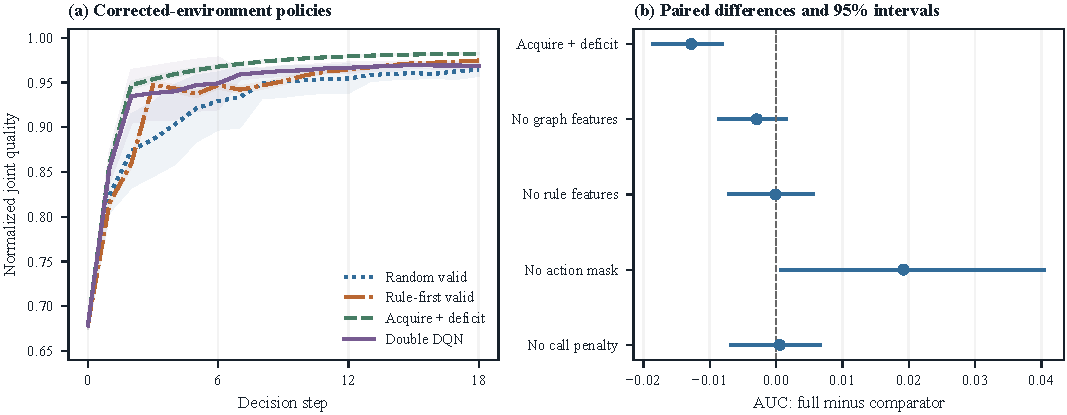
\includegraphics[width=0.98\textwidth]{figure/experiments/math_revision_policy.pdf}
\caption{Earlier count-penalty policy study on ten reused scenarios. (a) Mean evaluation quality with one-standard-deviation bands over ten scenarios. Terminal scores are carried forward to step 18. (b) Full Double DQN minus each comparator in AUC, with pointwise 95\% paired-bootstrap intervals. Multiplicity-adjusted tests appear in Table~\ref{tab:offline_tests}.}
\label{fig:rl_convergence}
\end{figure*}

\subsection{Retrained Component Ablations}
We train ten models for each of four variants, using the original 250 episodes per seed. The variants remove explicit graph features, explicit rule features, the action mask, or the acquisition-call penalty. Feature removal applies during both training and evaluation. The mask remains in the feature ablations and can convey rule availability. The no-mask variant removes masking from action selection and Bellman targets. The no-call-penalty variant changes only the training reward; evaluation uses the same corrected reward and cost coefficients for all settings.

\begin{table*}[t]
\centering
\caption{Component tests in the corrected environment. Each setting has ten retrained models.}
\label{tab:offline_ablations}
\footnotesize
\setlength{\tabcolsep}{3pt}
\begin{tabular*}{\textwidth}{@{\extracolsep{\fill}}lrrrrrr@{}}
\toprule
Setting & Final quality & AUC$_{18}$ & Calls & Invalid & New errors & Return \\
\midrule
Double DQN & $0.9686\pm0.0034$ & $0.9451\pm0.0096$ & 6.2 & 0.0 & 0.0 & 0.3660 \\
No graph features & $0.9713\pm0.0041$ & $0.9481\pm0.0028$ & 5.1 & 0.0 & 0.9 & 0.3693 \\
No rule features & $0.9692\pm0.0062$ & $0.9452\pm0.0034$ & 7.6 & 0.0 & 0.5 & 0.3594 \\
No action mask & $0.9480\pm0.0215$ & $0.9259\pm0.0278$ & 4.9 & 10.7 & 0.0 & 0.3430 \\
No call penalty & $0.9659\pm0.0051$ & $0.9446\pm0.0044$ & 8.1 & 0.0 & 0.0 & 0.3596 \\
\bottomrule
\end{tabular*}
\end{table*}

\begin{table*}[t]
\centering
\caption{Full Double DQN minus each baseline. Each interval is a paired-bootstrap 95\% CI. Holm correction covers ten tests.}
\label{tab:offline_tests}
\footnotesize
\setlength{\tabcolsep}{3pt}
\begin{tabular*}{\textwidth}{@{\extracolsep{\fill}}llrrr@{}}
\toprule
Baseline & Metric & Difference & 95\% interval & $p_{\mathrm{Holm}}$ \\
\midrule
Acquire + deficit & Final & -0.01392 & [-0.01604, -0.01205] & 0.0195 \\
Acquire + deficit & AUC & -0.01283 & [-0.01853, -0.00817] & 0.0195 \\
No graph features & Final & -0.00273 & [-0.00601, -0.00007] & 0.8340 \\
No graph features & AUC & -0.00292 & [-0.00862, +0.00151] & 1.0000 \\
No rule features & Final & -0.00068 & [-0.00406, +0.00268] & 1.0000 \\
No rule features & AUC & -0.00008 & [-0.00706, +0.00558] & 1.0000 \\
No action mask & Final & +0.02055 & [+0.00897, +0.03502] & 0.0195 \\
No action mask & AUC & +0.01921 & [+0.00075, +0.04042] & 0.8340 \\
No call penalty & Final & +0.00269 & [-0.00031, +0.00572] & 0.8340 \\
No call penalty & AUC & +0.00053 & [-0.00674, +0.00667] & 1.0000 \\
\bottomrule
\end{tabular*}
\end{table*}


Removing the mask lowers final quality to 0.94800 and produces 10.7 invalid actions per run. Its final-quality contrast passes Holm correction ($p=0.0195$); its AUC contrast does not ($p=0.8340$). The graph-feature, rule-feature, and call-penalty contrasts do not pass the ten-test correction. Thus the revised results support the action mask's contribution to final quality, while the other independent gains remain unestablished in this environment.

The analysis enumerates all $2^{10}$ sign assignments for exact two-sided paired randomization tests and applies Holm correction across ten contrasts: full Double DQN against the heuristic and four ablations, for both metrics. Pointwise intervals use 10,000 paired bootstrap draws. The sixty new models contribute 15,000 completed training episodes. Earlier checkpoints and results remain archived under their original environment version.

\section{Artifact Index}
\label{app:artifact_index}
Original checkpoints, transitions, and generation records remain under their original experiment directories. The earlier offline study is in \texttt{exps/paper2\_offline\_revision/}. It contains frozen source hashes, forty new checkpoints and training histories, all paired evaluation transitions, equal-call candidate samples, rule provenance, explicit label checks, and publication generators. The manuscript-to-artifact audit and offline reproduction commands accompany the results. These local analyses and training runs make zero API calls; the document-based generation requests are recorded separately.

The corrected environment, sixty retrained checkpoints, complete evaluation trajectories, shared-profile Paper1 revision, and rule bridge are in \texttt{exps/math\_revision\_20260925/}. Its source manifest and offline reproduction entry point accompany the results.

The reward-validation study is in \texttt{exps/paper2\_reward\_validation/}.
It contains training and test manifests, forty neural checkpoints, ten ridge
models and their public-feedback rollouts, development and test trajectories,
paired analyses, reconstruction checks, and generators for the active reward
figures and tables. Its README gives commands that require no API requests or
model downloads.

The separate policy-interface and coverage audit is in
\texttt{exps/paper2\_rule\_integration/}. It pins the raw CSV snapshots,
retains matching and nonmatching rules, and records sixteen schedule traces.
Public runtime records and scorer-only suite labels are stored separately.
Synthetic interface tests are excluded from empirical denominators.

\paragraph{Offline scheduling diagnosis.}
The follow-up in \texttt{exps/papers\_readiness\_20261002/} enumerates every
feasible acquisition, repair and stop sequence under the existing four-packet
budget and ten-step horizon. It preserves the two development rounds and
their twenty shared documents. References score paths only after enumeration.
Table~\ref{tab:offline_loop_ceiling} separates an executable schedule oracle
from a relaxed upper bound that may individually remove any injected record
reachable under the stored proposals.

\begin{table}[t]
\centering
\caption{All scheduling paths on the same ten development pairs per round. F1 averages pairs. Oracle scores use reference labels after replay.}
\label{tab:offline_loop_ceiling}
\footnotesize
\begin{tabular}{lrr}
\toprule
Diagnostic & Round 1 & Round 2 \\
\midrule
Feasible terminal paths & 363 & 235 \\
Stop F1 (\%) & 94.42 & 94.42 \\
Executable oracle F1 (\%) & 95.45 & 95.69 \\
Selective-removal upper F1 (\%) & 95.60 & 95.69 \\
Reward-optimal F1 (\%) & 91.63 & 95.69 \\
Oracle correct facts lost & 0 & 0 \\
Oracle injected items removed & 5 & 7 \\
\bottomrule
\end{tabular}
\end{table}


In round 1, the executable oracle reaches 95.45\% F1, but paths maximizing
the proxy reward reach 91.63\%, below stopping at 94.42\%. Wrong rules can
therefore misalign the proxy objective even with corrected reward accounting.
In round 2, both oracle bounds reach 95.69\%, equal to acquire-then-repair.
All seven removable injected items are covered by deletion-generated type
rules; augmentation and source constraints add no removal opportunities.
Once all packets are acquired and feasible repairs completed, round-2 final
graphs are identical across orders. Discounted returns still vary with order;
this leaves a cost and timing question, rather than additional final-F1
headroom on these fixed candidates. The 598 terminal paths are post-hoc
development diagnostics, not new documents or learned-policy evaluations.

An offline output-contract draft supplies separate legal enum examples,
explicit families, candidate limits and empty-result behavior. Replaying all
80 historical responses with the unchanged compiler reproduces their original
rules and rejections. The independent follow-up in
Appendix~\ref{app:new_rule_feasibility} subsequently freezes and tests a
version of this contract on other development documents. The old rounds
retain their original parser and scores.

\section{Supporting Repair-Layer Checks}
\label{app:supporting_checks}
These checks evaluate detector coverage, structural repair, and extraction
behavior. The learned-policy comparisons are reported in
Section~\ref{subsec:rl_results}; generated-rule effects are reported in
Section~\ref{subsec:generated_rule_transfer}.

\subsection{Separate Rule-Family Check}
\label{subsubsec:rule_family_final_ablation}
\begin{table}[t]
\centering
\caption{Hand-written family checks scored against stored suite labels. Table~\ref{tab:direct_execution} gives compiled generated patterns.}
\label{tab:rule_family_final_ablation}
\footnotesize
\setlength{\tabcolsep}{3pt}
\begin{tabular*}{\columnwidth}{@{\extracolsep{\fill}}lrrrrr@{}}
\toprule
Detector & TP & FP & FN & Recall & F1 \\
\midrule
Deletion-family & 34 & 0 & 30 & 0.531 & 0.694 \\
Augmentation-family & 30 & 0 & 34 & 0.469 & 0.638 \\
Family union & 64 & 0 & 0 & 1.000 & 1.000 \\
\bottomrule
\end{tabular*}
\end{table}

The hand-implemented deletion-family detector covers 34 procedural, missing-field, and specialist defects. The augmentation-family detector covers the other 30 structural defects. Their union detects all 64 defects with no false positives when scored against the stored expected labels. These functions encode the designed defect families directly. Their coverage establishes a regression check for those families; the direct execution results in Table~\ref{tab:direct_execution} measure the archived generated patterns.

\subsection{Comparison with Constraint-Checking Baseline}
\label{subsec:shacl_baseline}

We compare with a deterministic constraint-checking baseline implemented with SHACL-style RDF validation. This baseline receives deduplicated RDF triples and checks schema-conformance constraints, but it does not access the source text, LLM prompts, or generated procedural/value rules. This comparison measures the coverage of the selected shapes on these inputs.

\begin{table}[t]
    \centering
    \caption{SHACL-style structural validation baseline on three domains.}
    \label{tab:shacl_baseline}
    \footnotesize
    \setlength{\tabcolsep}{2pt}
    \begin{tabular*}{\columnwidth}{@{\extracolsep{\fill}}l r r c c@{}}
    \toprule
    Domain & Raw Triples & RDF Dedup. & Removed & $Q$ \\
    \midrule
    Gov. Affairs & 13,892 & 10,771 & 0 & 79.87 \\
    Finance & 2,264 & 539 & 0 & 70.42 \\
    Env. & 2,345 & 378 & 0 & 65.25 \\
    \midrule
    Average & 6,167 & 3,896 & 0 & 71.85 \\
    \bottomrule
    \end{tabular*}
\end{table}

The inputs conform to the selected shapes after RDF deduplication, so the baseline removes no additional triples. Its average quality score is 71.85 under the separate quality metric. These shapes do not implement all source-dependent and procedural checks used by that metric. This is a difference in implemented constraint coverage; SHACL can express richer value and logical constraints than this baseline uses.

\subsection{Deterministic Structural Repair}
\label{subsec:external_benchmark}

A separate deterministic benchmark uses TNEWS/CLUE-style Chinese news titles. A deterministic extractor constructs a document--category--entity KG from 3,000 balanced news titles across 15 categories; we then inject duplicate triples, invalid relations, and isolated nodes, and run the local repair pipeline. This benchmark is fully local and makes no LLM/API calls, so it evaluates KG quality control and rule execution rather than LLM extraction quality.

\begin{table}[t]
    \centering
    \caption{TNEWS/CLUE local end-to-end KG quality benchmark.}
    \label{tab:tnews_external_benchmark}
    \footnotesize
    \setlength{\tabcolsep}{2pt}
    \begin{tabular*}{\columnwidth}{@{\extracolsep{\fill}}l c c c c@{}}
    \toprule
    Stage & Nodes & Relations & Invalid & $Q$ \\
    \midrule
    Clean extraction & 10,871 & 20,827 & 0.000 & 99.89 \\
    Corrupted KG & 11,414 & 22,909 & 0.050 & 94.93 \\
    Repaired KG & 10,822 & 19,799 & 0.000 & 100.00 \\
    \bottomrule
    \end{tabular*}
\end{table}

The repair pipeline removes injected invalid relations, duplicate triples, and isolated noise nodes, improving structural $Q$ from 94.93 to 100.00. The repaired graph has fewer nodes and relations than the clean extraction, so this score does not mean that every original fact was recovered. The full report is generated by \texttt{exps/external\_benchmark\_runner.py}.

\subsection{API-Backed LLM Extraction Benchmark}
\label{subsec:api_llm_benchmark}

The local TNEWS/CLUE benchmark above isolates the quality-control layer under deterministic extraction. To additionally test the full extraction path, the archived API benchmark evaluated on 45 TNEWS/CLUE titles covering 15 categories. The model is Qwen3.8-27B-no-thinking. TNEWS category labels are used as silver labels for category inference, and provided title keywords are used as weak silver mentions for entity coverage. The test measures parsing, weak extraction indicators, and structural filtering of model outputs.

\begin{table}[t]
    \centering
    \caption{API-backed LLM extraction benchmark on TNEWS/CLUE titles.}
    \label{tab:api_llm_benchmark}
    \footnotesize
    \setlength{\tabcolsep}{2pt}
    \begin{tabular*}{\columnwidth}{@{\extracolsep{\fill}}l c c@{}}
    \toprule
    Metric & Raw LLM KG & Repaired KG \\
    \midrule
    Parse success & 1.000 & --- \\
    Category accuracy & 0.556 & 0.556 \\
    Keyword recall & 0.178 & 0.178 \\
    Documents with triples & 1.000 & 1.000 \\
    Avg. triples / doc & 3.58 & 3.58 \\
    Invalid triple rate & 0.000 & 0.000 \\
    Duplicate triple rate & 0.000 & 0.000 \\
    KG quality score & 100.00 & 100.00 \\
    \bottomrule
    \end{tabular*}
\end{table}

The 45 calls completed in 1,190.90 seconds and all responses parsed successfully. Qwen3.8-27B-no-thinking followed the allowed schema on every sampled title, so the conservative repair layer made no change: raw and repaired structural quality are both 100.00. No structural violation was detected on this sample. Category accuracy is 0.556 and weak keyword recall is 0.178, indicating that semantic extraction remains the larger bottleneck; deterministic structural checks cannot repair omitted or misclassified content.


\section{Bridge Coverage and Runtime Records}
\label{app:bridge_coverage}
\subsection{Types and Fixed-Schedule Traces}
The bridge in Section~\ref{sec:rule_bridge_method} provides a public-observation interface for loading either strategy's archived rule bank, removing unopposed forbidden matches, or stopping. Two acquisition orders, each with immediate or deferred removal, give four schedules per input. Across RuleTest-94 and three archived graph snapshots, we retain sixteen complete action traces. All four schedules remove the same ten designed defects and no clean record on RuleTest-94. No late permission or conflict occurs in these empirical replays. Separate synthetic tests verify conflict abstention and log a permission that arrives after a record was removed; those tests do not add empirical cases.


The original government, finance and environment CSV snapshots contain 17,939, 8,180 and 151 edge occurrences, respectively. Their node types are all \texttt{Unknown}, leaving 26,270 edges without the type information required by the archived patterns. A further provenance audit checks 51 tracked node CSV files, the three original document JSONL files and two separate-task extraction checkpoints. It restores no traceable types for these graphs. In the enhanced exports, \texttt{Enhanced} is assigned by the converter as a processing tag, not an entity class; numeric IDs alone do not establish identity across exports. The runtime abstains on these records. Table~\ref{tab:rule_integration_coverage} distinguishes this missing information from the absence of a matching rule on typed records. These are separately pinned raw snapshots, not the inputs of the SHACL comparison in Appendix~\ref{subsec:shacl_baseline}.

On RuleTest-94, the two matching patterns both come from deletion: one permission matches ten records and one prohibition flags another ten. Augmentation matches no record. The resulting coverage and identical final records across schedules identify the next integration requirement: trusted entity types and broader applicable rule coverage before testing learned scheduling. The replay interface provides no reward and uses no learned checkpoints. Loading a strategy bank is reported as loading 4,728 archived responses, with zero actual API requests.

\subsection{Runtime Details}
\label{app:runtime_details}
The original twenty-model RL run recorded 1,278.99 seconds of CPU time with zero API calls. The earlier sixty-model component study and the new forty-model reward study also make zero requests. The new ridge controls add ten fits from 2,500 random exploration episodes. The current-reward component and small-count study adds fifty trained models, again with zero API requests. Per-run training durations and evaluation timings are archived. Evaluation timing covers policy inference and environment transitions, excluding environment construction. Model-informed lookahead additionally includes cloned transition probes. These local timings do not estimate LLM latency.

The earlier 45-document extraction test made 45 actual calls and recorded 1,190.90 seconds. The rule archive records 9,456 successful responses; historical latency, tokens, retries, and failed requests are not fully recorded. Equal-call candidate comparisons therefore measure diversity per archived successful call, rather than total billed cost. The environment's acquisition units model that cost during scheduling.
